\documentclass[tikz,border=2pt]{standalone}
\usepackage{amsmath}
\usetikzlibrary{arrows.meta}
\begin{document}
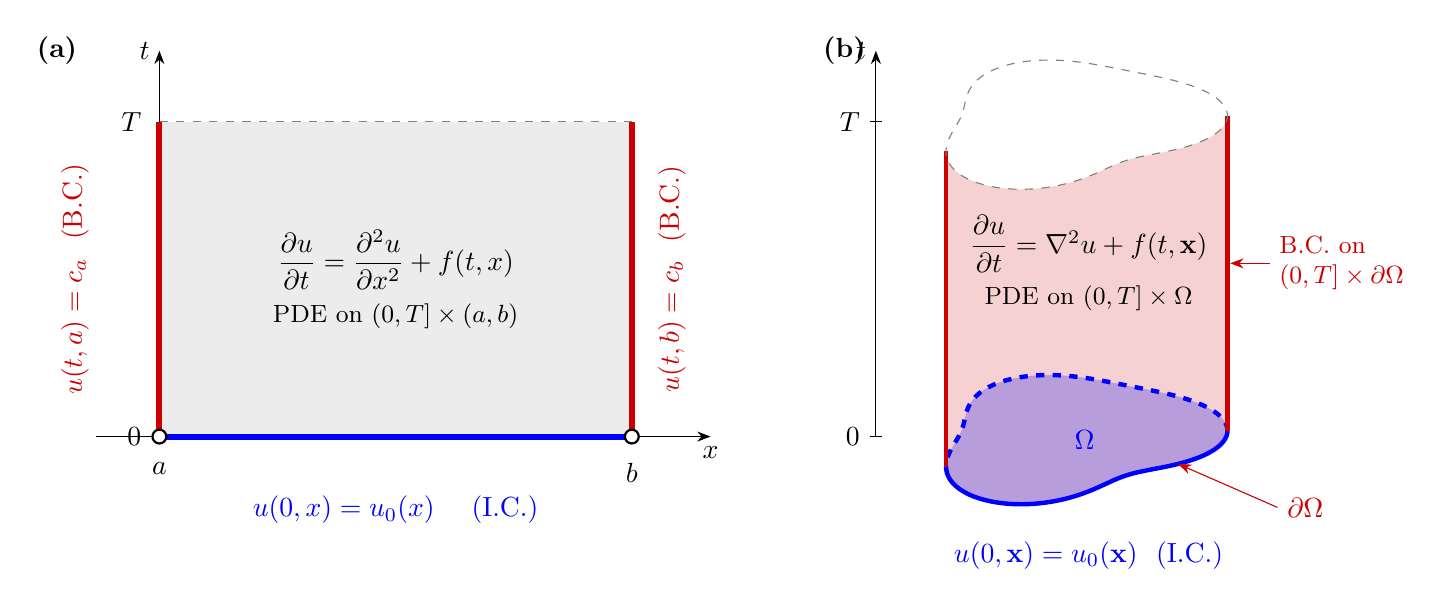
\begin{tikzpicture}[scale=1.0, >=Stealth]
% ---------------- (a) 1D space-time domain (0,T] x (a,b) ----------------
\begin{scope}
    \def\a{0} \def\b{6} \def\T{4}
    % interior: where the PDE is imposed
    \fill[gray!15] (\a,0) rectangle (\b,\T);
    \draw[gray, thin, dashed] (\a,\T) -- (\b,\T);
    % axes
    \draw[->] (-0.8,0) -- (\b+1.0,0) node[below] {$x$};
    \draw[->] (\a,0) -- (\a,\T+0.9) node[left] {$t$};
    % tick labels
    \node[below=6pt] at (\a,0) {$a$};
    \node[below=6pt] at (\b,0) {$b$};
    \node[left=3pt] at (\a,\T) {$T$};
    \node[left=3pt] at (\a,0) {$0$};
    % initial condition on {t = 0} x (a,b)
    \draw[line width=2.2pt, blue] (\a,0) -- (\b,0);
    % boundary conditions on (0,T] x {a} and (0,T] x {b}
    \draw[line width=2.2pt, red!80!black] (\a,0) -- (\a,\T);
    \draw[line width=2.2pt, red!80!black] (\b,0) -- (\b,\T);
    % corners (0,a), (0,b) are excluded from both the I.C. and the B.C.
    \filldraw[fill=white, draw=black, thick] (\a,0) circle (2.5pt);
    \filldraw[fill=white, draw=black, thick] (\b,0) circle (2.5pt);
    % PDE label
    \node[align=center] at ({(\a+\b)/2},{\T/2})
        {$\dfrac{\partial u}{\partial t} = \dfrac{\partial^2 u}{\partial x^2} + f(t,x)$\\[4pt]
         \small PDE on $(0,T] \times (a,b)$};
    % I.C. label
    \node[blue, below=18pt, align=center] at ({(\a+\b)/2},0)
        {$u(0,x) = u_0(x)$ \quad (I.C.)};
    % B.C. labels
    \node[red!80!black, rotate=90, above=22pt] at (\a,{\T/2})
        {$u(t,a) = c_a$ \ (B.C.)};
    \node[red!80!black, rotate=90, below=6pt] at (\b,{\T/2})
        {$u(t,b) = c_b$ \ (B.C.)};
    \node[font=\bfseries] at (-1.3,\T+0.9) {(a)};
\end{scope}

% ---------------- (b) space-time cylinder (0,T] x Omega ----------------
\begin{scope}[xshift=11.6cm]
    \def\H{4}
    % boundary curve of Omega: R(th) = 1.7 + 0.25 cos 3th + 0.18 sin 2th,
    % drawn in oblique projection (x2 squashed by 0.45)
    \def\bx(#1){(1.7+0.25*cos(3*#1)+0.18*sin(2*#1))*cos(#1)}
    \def\by(#1){0.45*(1.7+0.25*cos(3*#1)+0.18*sin(2*#1))*sin(#1)}
    % silhouette angles (extreme x): th = 207.6 (left), 364.84 (right)
    % lateral surface (0,T] x dOmega: boundary conditions
    \fill[red!80!black, opacity=0.18]
        plot[domain=207.6:364.84, samples=80, smooth] ({\bx(\x)},{\by(\x)})
        -- plot[domain=364.84:207.6, samples=80, smooth] ({\bx(\x)},{\by(\x)+\H})
        -- cycle;
    % base {0} x Omega: initial condition
    \fill[blue, opacity=0.25]
        plot[domain=0:360, samples=160, smooth cycle] ({\bx(\x)},{\by(\x)});
    \draw[line width=1.6pt, blue, dashed]
        plot[domain=4.84:207.6, samples=80, smooth] ({\bx(\x)},{\by(\x)});
    \draw[line width=1.6pt, blue]
        plot[domain=207.6:364.84, samples=80, smooth] ({\bx(\x)},{\by(\x)});
    % silhouette lines
    \draw[line width=1.6pt, red!80!black] (-1.6098,-0.3787) -- (-1.6098,-0.3787+\H);
    \draw[line width=1.6pt, red!80!black] (1.9652,0.0749) -- (1.9652,0.0749+\H);
    % top {T} x Omega: nothing imposed
    \draw[gray, thin, dashed]
        plot[domain=0:360, samples=160, smooth cycle] ({\bx(\x)},{\by(\x)+\H});
    % time axis
    \draw[->] (-2.5,0) -- (-2.5,\H+0.9) node[left] {$t$};
    \draw (-2.58,0) -- (-2.42,0) node[pos=0, left] {$0$};
    \draw (-2.58,\H) -- (-2.42,\H) node[pos=0, left] {$T$};
    % labels
    \node[align=center] at (0.2,{\H/2+0.2})
        {$\dfrac{\partial u}{\partial t} = \nabla^2 u + f(t,\mathbf{x})$\\[4pt]
         \small PDE on $(0,T] \times \Omega$};
    \node[blue] at (0.15,-0.05) {$\Omega$};
    \node[blue, below=10pt, align=center] at (0.2,-0.86)
        {$u(0,\mathbf{x}) = u_0(\mathbf{x})$ \ (I.C.)};
    \draw[red!80!black, <-] (2.0,{\H*0.55}) -- (2.5,{\H*0.55})
        node[right, align=left, font=\small]
        {B.C. on\\$(0,T] \times \partial\Omega$};
    \draw[red!80!black, <-] ({\bx(330)},{\by(330)}) -- (2.6,-0.9)
        node[right] {$\partial\Omega$};
    \node[font=\bfseries] at (-2.9,\H+0.9) {(b)};
\end{scope}
\end{tikzpicture}
\end{document}
